\chapter{Progettazione e codifica}
\label{cap:progettazione-codifica}

\intro{Il capitolo inizialmente presenta gli strumenti e le tecnologie analizzate e utilizzate per la realizzazione del prodotto. Successivamente si vede l'effettiva creazione delle classi del progetto, affiancate da una struttura preesistente fondamentale per le classi affinché il modulo funzioni e svolga la sua funzione. }\\

\section{Tecnologie e strumenti}
\label{sec:tecnologie-strumenti}

Di seguito viene data una panoramica delle tecnologie e strumenti utilizzati.

\subsection*{HTML5}
Tecnologia standard per la creazione di pagine web. Studiata attraverso il corso di Tecnologie Web.

\subsection*{CSS}
Tecnologia standard per la creazione di pagine web e il loro abbellimento. Fornisce una vasta gamma di funzionalità per la personalizzazione delle pagine. Studiata attraverso il corso di Tecnologie Web.
\subsection*{Bootstrap3/5}
Bootstrap è un framework che fornisce delle classi le quali raggruppano uno o più attributi del css, per la creazione di pagine web \textit{responsive\gls}. \\
Bootstrap è utilizzato nello stile \textit{inline} di \textit{HTML} e le sue classi vengono inserite all'interno del \textit{tag\gls} "class" di HTML di un elemento. In questo modo, specificando la classe di Boostrap che si vuole utilizzare, verrà applicato un certo stile all'elemento selezionato. Si possono concatenare più classi per un certo elemento.\\
La differenza tra le due versioni di \textit{Boostrap} 3 e 5 è nella gamma di funzionalità che offrono. La versione 5 è la più recente e molte più funzionalità di quelle precedenti, adattandosi alle nuove feature di \textit{HTML5}. \\
Ad oggi si cerca di migrare dalle versioni più vecchie a quella più recente.
\subsection*{Servlet}
Le \textit{servlet} permettono di soddisfare delle \textit{request\gls} \textit{HTTP\gls} proveniente da web. Ogni servlet viene richiamata e caricata una sola volta e poi resta in memoria per rispondere alle chiamate successive. 
\subsection*{JSP}
Le \textit{JavaServer Page} rappresentano una tecnologia fondamentale per la realizzazione di pagine web dinamiche. Infatti forniscono dei \textit{tag} speciali con i quali possono essere richiamate delle funzioni specifiche in modo da rendere la pagina dinamica. I file \textit{JSP} sono caratterizzati dell'estensione .jsp e costituiscono le vere e proprie pagine web visualizzate dall'utente; infatti sono codificate in \textit{HTML} e \textit{XML}.
\subsection*{JSTL}
\textit{JavaServer Pages Standard Tag Library} è una libreria che estende JSP offrendo nuove funzionalità per applicazioni web in \texit{JAVA EE}. 
\subsection*{Apache Struts}
\textit{Apache Struts} è un \textit{framework oper-source} che supporta lo sviluppo di applicazioni web in Java con il pattern MVC. \textit{Struts} ha il compito di organizzare le richieste del client e richiamare le funzionalità della logica di business. \\
Il framework è composto da tre elementi principali:
\begin{itemize}
\item \textit{Request Handler\gls}: viene mappato ad un URI dallo sviluppatore;
\item \textit{Response Handler\gls}: la risposta verrà passata ad un'altra risorsa che la completerà;
\item \textit{Tag}: aiutano lo sviluppatore per lo sviluppo.
\end{itemize}

\noindent
Per configurare tutti i collegamenti tra i vari elementi e le loro interazioni si utilizza il file \textit{\textbf{struts.xml}}. In questo file vengono specificati anche gli \textit{\textbf{interceptor}} per le \textit{Action} delle nostre classi. La specifica degli \textit{interceptor} è una fase importante dello sviluppo di un'applicazione web.

\subsection*{JQUERY Taconite}
\textit{JQUERY Taconite} permette di aggiornare \texit{DOM} multipli utilizzando il risultato di una singola chiamata \textit{AJAX\gls}. \\
Viene generato un \textit{XML} con le istruzioni per l'aggiornamento dei diversi \textit{DOM}.

\subsection*{Hibernate}
È un framework che permette di mappare gli oggetti del modello ad un \textit{database} relazionale. Lo sviluppatore non deve preoccuparsi di implementazione ma è \textit{Hibernate} che si occupa del collegamento al database e di eseguire le operazioni \textit{CRUD\gls}, andando a generare query e leggerne il risultato.

\subsection*{Spring}
\textit{Spring}\gls è un framework volto ad aiutare lo sviluppo di applicazioni più o meno complesse attraverso la sua architettura modulare. Spring è diviso in cinque livelli e in questo modo si possono escludere le parti non necessarie per l'applicazione.\\
L'elemento principale di \textit{Spring} è il \textit{Core Container} che ha il compito di creazione e gestione di tutti gli oggetti dell'applicazione, detti anche \textit{\textbf{beans}\gls}.
\subsection*{Wro4j}
\textit{Wro4j} è uno strumento per l'ottimizzare le risorse web e velocizzare il caricamento delle pagine. Il suo compito è quello di organizzare le risorse, come i file \textit{css} e \textit{js}, raggrupparli e farli scaricare tutti in una sola volta alla pagina web.\\
Normalmente un browser può scaricare al massimo due risorse contemporaneamente e questo limite porta ad un caricamento della pagina lento in vista di molte risorse da scaricare. \textit{Wro4j} elimina questo problema comprendendo tutte le risorse in un'unica risorsa.
\subsection*{SVNKit}
\textit{SVNKit} è uno \textit{toolkit} \textit{Open-Source} e permette l'accesso il remoto e in locale a delle \textit{repository} per le applicazioni Java. Funge anche da sistema di versionamento. 

\subsection*{Apache Maven}
\textit{Apache Maven} è uno strumento per la gestione delle dipendenze tra un progetto Java e le versioni delle librerie che servono e si occupa anche di effettuare il download di tali risorse. \\
Le relazioni tra progetto e librerie sono definite in un file \textit{XML} chiamato \textit{\textbf{pom.xml}}.

\subsection*{Apache Tomcat}
\textit{Apache Tomcat} è un server web che permette l'esecuzione di applicazioni web. Supporta le specifiche di \textit{JSP} e \textit{servlet}.\\
Esistono diverse versioni per i server \textit{Tomcat} e si può scegliere la versione che offre le funzionalità giuste per la propria applicazione.
\subsection*{DBeaver}
È un'applicazione che si occupa di gestire i database. Si possono creare nuovi database, creare tabelle, manipolare i dati, ecc...

\section{Progettazione}
\label{sec:progettazione}
La fase di progettazione era una fase cruciale per la realizzazione del progetto. Prima ancora di iniziare la progettazione del lavoro assegnato è stato importante analizzare l'ambiente già esistente, capirne il funzionamento e individuare se c'erano elementi che potevano servire al nostro scopo. \\
Una tecnica per una buona progettazione è stata concentrarsi su un elemento alla volta. Prendere in considerazione tutti gli elementi del progetto poteva sembrare più efficace e veloce, ma così facendo si avremmo perso il focus della funzione delle classi del prodotto.\\ 
Quindi l'idea era di analizzare e progettare una singola classe, controllarne il corretto funzionamento e da lì procedere ed andare avanti con lo studio per la realizzazione delle prossime classi.


\subsection{Base di Dati}
Per la progettazione della base di dati sono iniziato da un database già esistente nell'azienda e ho inserito i nuovi elementi del progetto. Poi ho eseguito un \textit{refactoring} di alcune delle tabelle preesistenti per correggerle ed adattarle a quelle nuove, senza però modificarne attributi fondamentali per le altre parti della webapp. Anche qui c'è stata allora una fase di profonda e attenta analisi per avere una base di dati consistente. 
\subsubsection*{Tabelle preesistenti}
Il progetto utilizzava tabelle preesistenti per il suo scopo. Le tabelle erano le seguenti: 
\begin{itemize}


    \item \textbf{Cliente}: questa tabella rappresentava l'entità cliente e aveva tutti gli attributi necessari per definirne lo scopo all'interno della webapp. Il cliente non era la singola persona ma bensì l'azienda a cui poi erano collegati sia i dipendenti sia i progetti richiesti da questa. Alcuni attributi presenti servono per le altre componenti della webapp;
    \item \textbf{User}: gli user erano tutte le persone coinvolte nell'azienda, interne ed esterne. Quindi la tabella comprendeva sia il personale di CWBI sia il personale delle aziende clienti;
    \item \textbf{Progetto}: questa tabella rappresentava un progetto dell'azienda. Aveva tutti gli attributi necessari ed era collegata ad un cliente. Un progetto poteva essere collegato a più aziende diverse;
    \item \textbf{ProgettoCliente}: questa tabella rappresentava la relazione tra progetto e cliente. Veniva chiamata in causa quando si doveva scegliere l'azienda e il progetto su cui si voleva aprire il ticket;
        \item \textbf{ProgettoUser}: questa tabella rappresentava la relazione tra progetto e user. Ad ogni progetto si potevano associare uno o più utenti.
\end{itemize}

\subsubsection*{Tabelle introdotte}
\begin{itemize}
	\item \textbf{Ticket}: questa tabella rappresentava l'entità ticket con tutti gli attributi che lo caratterizzavano. Aveva un collegamento all'entità ProgettoCliente in quanto il ticket era aperto per uno specifico progetto di una specifica azienda.
	
	\item \textbf{TicketItem}: questa tabella rappresentava i commenti presenti in ogni ticket. Un commento poteva avere un solo ticket di riferimento, cioè quello in cui è stato scritto.
\end{itemize}


\begin{figure}[H]
\bigskip
\bigskip
\bigskip
\bigskip
    \centering 
    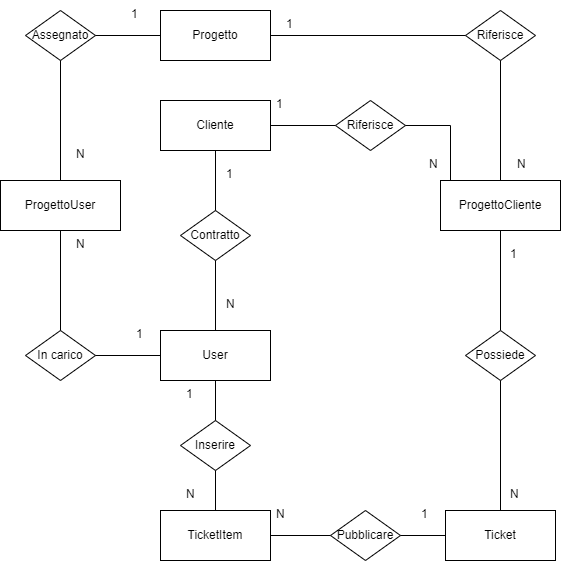
\includegraphics[width=1.1\columnwidth]{diagrammaBase} 
    \bigskip
    \caption{Base di Dati - Relazioni delle tabelle del progetto}
\end{figure}

\newpage

\begin{figure}[H]
\bigskip
\bigskip
\bigskip
\bigskip
\bigskip
    \centering 
    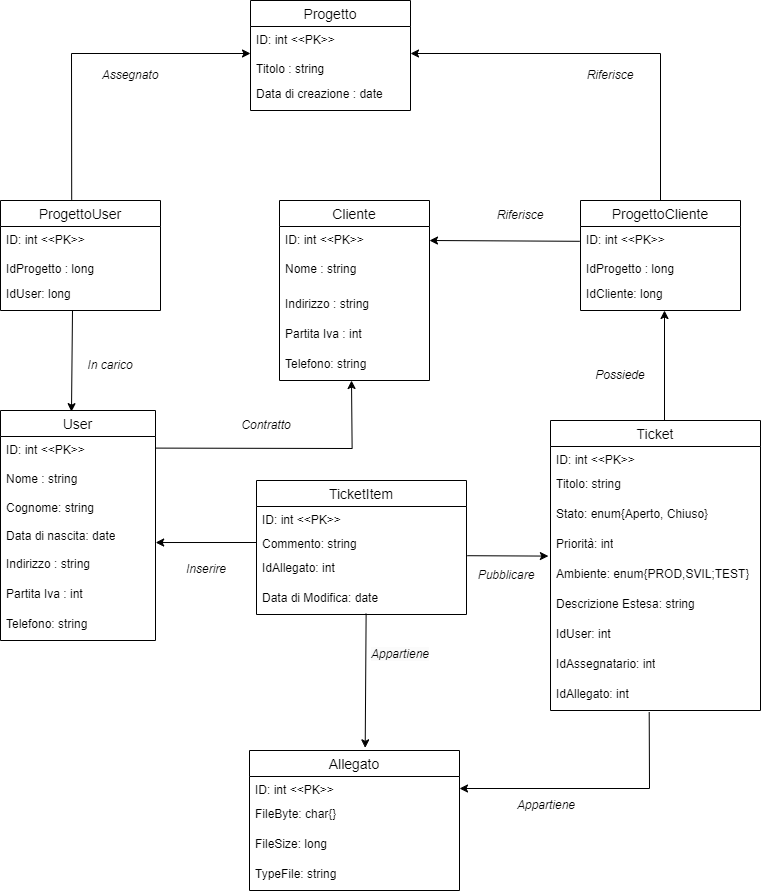
\includegraphics[width=1.1\columnwidth]{diagrammaEvoBase} 
    \bigskip
    \caption{Base di Dati - Tabelle del progetto}
\end{figure}
\newpage

\subsubsection*{Analisi delle tabelle}
            \begin{table}[H]
                \centering
                \renewcommand{\arraystretch}{1.8}
                \renewcommand\tabularxcolumn[1]{m{#1}}
                \begin{tabularx}{0.9\textwidth} {
                    >{\hsize=.8\hsize\linewidth=\hsize}X
                    >{\hsize=1.2\hsize\linewidth=\hsize}X}
                    \textbf{Cliente}\\
                    \hline
                    \textit{Id} & Identificativo univoco di ogni cliente. \\
                    \hline
                    \textit{Nome} & Nome dell'azienda.  \\
                    \hline
                    \textit{Indirizzo} & Indirizzo della sede principale dell'azienda. \\
                    \hline
                    \textit{Partita Iva} & Partita Iva dell'azienda \\
                    \hline
   	                \textit{Telefono} & Telefono dell'azienda \\
                    \hline
                \end{tabularx}
                \smallskip
                \caption{Tabella Cliente}
            \end{table}
            \smallskip
 \begin{table}[H]
                \centering
                \renewcommand{\arraystretch}{1.8}
                \renewcommand\tabularxcolumn[1]{m{#1}}
                \begin{tabularx}{0.9\textwidth} {
                    >{\hsize=.8\hsize\linewidth=\hsize}X
                    >{\hsize=1.2\hsize\linewidth=\hsize}X}
                    \textbf{ProgettoCliente}\\
                    \hline
                    \textit{Id} & Identificativo univoco di ogni ProgettoCliente. \\
                    \hline
                    \textit{IdProgetto} & Id del progetto a cui si riferisce.  \\
                    \hline
                    \textit{IdCliente} & Id dell'azienda a cui si riferisce. \\
                    \hline
                \end{tabularx}
                \smallskip
                \caption{Tabella ProgettoCliente}
            \end{table}
            \smallskip
 \begin{table}[H]
                \centering
                \renewcommand{\arraystretch}{1.8}
                \renewcommand\tabularxcolumn[1]{m{#1}}
                \begin{tabularx}{0.9\textwidth} {
                    >{\hsize=.8\hsize\linewidth=\hsize}X
                    >{\hsize=1.2\hsize\linewidth=\hsize}X}
                    \textbf{Progetto}\\
                    \hline
                    \textit{Id} & Identificativo univoco di ogni Progetto. \\
                    \hline
                    \textit{Titolo} & Titolo del progetto.  \\
                    \hline
                    \textit{Data di creazione} & Data in cui è stato aperto il progetto. \\
                    \hline
                \end{tabularx}
                \smallskip
                \caption{Tabella Progetto}
            \end{table}
            \smallskip

 \begin{table}[H]
                \centering
                \renewcommand{\arraystretch}{1.8}
                \renewcommand\tabularxcolumn[1]{m{#1}}
                \begin{tabularx}{0.9\textwidth} {
                    >{\hsize=.8\hsize\linewidth=\hsize}X
                    >{\hsize=1.2\hsize\linewidth=\hsize}X}
                    \textbf{ProgettoUser}\\
                    \hline
                    \textit{Id} & Identificativo univoco di ogni ProgettoUser. \\
                    \hline
                    \textit{IdProgetto} & Id del progetto a cui si riferisce.  \\
                    \hline
                    \textit{IdUser} & Id dell'utente a cui si riferisce. \\
                    \hline
                \end{tabularx}
                \smallskip
                \caption{Tabella ProgettoUser}
            \end{table}   
                 
    			\smallskip 
            \begin{table}[H]
                \centering
                \renewcommand{\arraystretch}{1.8}
                \renewcommand\tabularxcolumn[1]{m{#1}}
                \begin{tabularx}{0.9\textwidth} {
                    >{\hsize=.8\hsize\linewidth=\hsize}X
                    >{\hsize=1.2\hsize\linewidth=\hsize}X}
                    \textbf{User}\\
                    \hline
                    \textit{Id} & Identificativo univoco di ogni User. \\
                    \hline
                    \textit{Nome} & Nome dell'utente.  \\
                    \hline
                    \textit{Cognome} & Cognome dell'utente.  \\
                    \hline
                     \textit{Data di nascita} & Data di nascita dell'utente.  \\
                    \hline
                    \textit{indirizzo} & Indirizzo dell'utente.  \\
                    \hline
                    \textit{Partita Iva} & Partita Iva dell'utente \\
                    \hline
   	                \textit{Telefono} & Telefono dell'utente \\
                    \hline
                \end{tabularx}
                \smallskip
                \caption{Tabella User}
            \end{table}
            \smallskip 
            
 \begin{table}[H]
                \centering
                \renewcommand{\arraystretch}{1.8}
                \renewcommand\tabularxcolumn[1]{m{#1}}
                \begin{tabularx}{0.9\textwidth} {
                    >{\hsize=.8\hsize\linewidth=\hsize}X
                    >{\hsize=1.2\hsize\linewidth=\hsize}X}
                    \textbf{Ticket}\\
                    \hline
                    \textit{Id} & Identificativo univoco di ogni Ticket. \\
                    \hline
                    \textit{Titolo} & Titolo del ticket.  \\
                    \hline
                    \textit{Stato} & Stato del Ticket. \\
                    \hline
                    \textit{Priorità} & Priorità che un ticket ha. Parte da un minimo di 1, quindi poco urgente, ad un massimo di 4, urgente. \\
                    \hline            
            
                 \end{tabularx}
                \smallskip
                \caption{Tabella Ticket}
            \end{table}  
            
 \begin{table}[H]
                \centering
                \renewcommand{\arraystretch}{1.8}
                \renewcommand\tabularxcolumn[1]{m{#1}}
                \begin{tabularx}{0.9\textwidth} {
                    >{\hsize=.8\hsize\linewidth=\hsize}X
                    >{\hsize=1.2\hsize\linewidth=\hsize}X}
                    \hline
                    \textit{Ambiente} & Ambiente del Ticket. Un ticket può essere aperto in base all'ambiente in cui si sta testando l'applicazione e si trova il problema. Si hanno tre diversi ambienti: PROD, SVIL, TEST.\\
                    \hline
                    \textit{Descrizione} & Descrizione del Ticket. Utile per approfondire il problema che si è riscontrato.\\
                    \hline
                    \textit{IdUser} & Id dell'utente che ha aperto il ticket. \\
                    \hline
                    \textit{IdAssegnatario} &  Id dell'utente a cui è stato assegnato il ticket. Può essere cambiato durante il ciclo di vita del ticket. \\
                
                    \hline
                   \textit{IdAllegato} &  Id dell'allegato caricato al ticket. Può essere cambiato durante il ciclo di vita del ticket. \\
                
                    \hline
                \end{tabularx}
                \smallskip
                \caption{Tabella Ticket}
            \end{table}   
                 
    			\smallskip      

 \begin{table}[H]
                \centering
                \renewcommand{\arraystretch}{1.8}
                \renewcommand\tabularxcolumn[1]{m{#1}}
                \begin{tabularx}{0.9\textwidth} {
                    >{\hsize=.8\hsize\linewidth=\hsize}X
                    >{\hsize=1.2\hsize\linewidth=\hsize}X}
                    \textbf{TicketItem}\\
                    \hline
                     \textit{Id} & Identificativo univoco di ogni Commento. \\
                    \hline
                    \textit{Commento} & Contenuto del commento. \\
                    \hline
                    \textit{IdAllegato} & Id dell'allegato caricato al commento. \\
                    \hline
                    \textit{Data di Modifica} & Data in cui è stato modificato il ticket. \\
                    \hline
                \end{tabularx}
                \smallskip
                \caption{Tabella TicketItem}
            \end{table}
            \smallskip
            
 \begin{table}[H]
                \centering
                \renewcommand{\arraystretch}{1.8}
                \renewcommand\tabularxcolumn[1]{m{#1}}
                \begin{tabularx}{0.9\textwidth} {
                    >{\hsize=.8\hsize\linewidth=\hsize}X
                    >{\hsize=1.2\hsize\linewidth=\hsize}X}
                    \textbf{Allegato}\\
                    \hline
                    \textit{FileByte} & Contenuto del file caricato codificato in un vettore di caratteri (char[]) \\
                    \hline
                    \textit{FileSize} & Dimensione del file caricato. \\
                    \hline
                    \textit{TypeFile} & Tipo del file caricato. \\
                    \hline
                \end{tabularx}
                \smallskip
                \caption{Tabella Allegato}
            \end{table}
            
\newpage
\subsection{Architettura}
Lo sviluppo dell'applicazione è avvenuta secondo il \textit{pattern} architetturale \textbf{MVC \glsfirstoccur} (\textit{Model - View - Controller}). \\
Questo \textit{pattern} permette di dividere e rendere modulabile l'applicazione.
\begin{itemize}
\item \textbf{Model}: si occupa della gestione dei dati, del salvataggio delle risorse e della logica di business;
\item \textbf{View}: si occupa di visualizzare i dati salvati nel modello, presentandoli secondo una schema definito;
\item \textbf{Controller}: ha il compito di gestire la comunicazione tra il modello e la vista ed elaborare gli input dell'utente per poi fornire in output un determinato risultato.
\end{itemize}

\begin{figure}[H]
    \centering 
    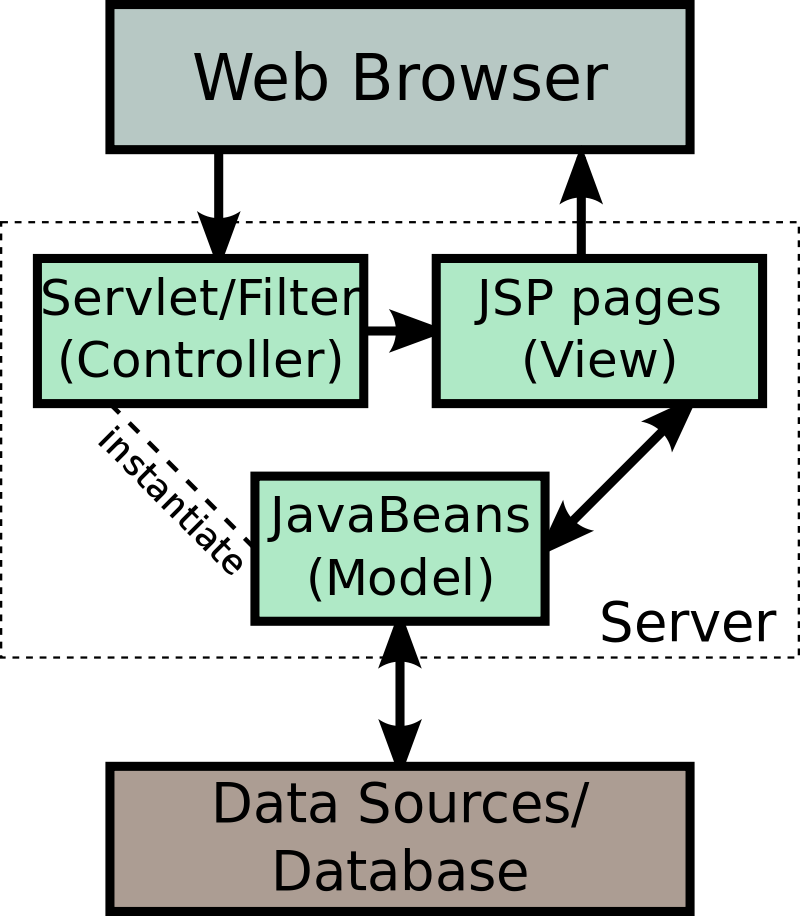
\includegraphics[width=0.4\columnwidth]{MVC} 
    \bigskip
    \caption{Schema MVC}
\end{figure}

\noindent
Utilizzare il pattern \textit{MVC} permette di avere dei \textbf{vantaggi}:
\begin{itemize}
\item \textbf{Manutenzione}: la suddivisione in componenti rende la manutenzione dell'applicazione più semplice, andando a concentrarsi sulla parte interessata;
\item \textbf{Scalabilità}: con l'aumentare delle esigenze l'applicazione richiederà degli aggiornamenti che saranno meglio integrabili;
\item \textbf{Testabilità}: senza il pattern \textit{MVC}, per eseguire il test su un parte dell'applicazione, bisognerebbe eseguire la diagnosi sul complessivo. Mentre la suddivisione in componenti permette di eseguire i test più velocemente prendendo in considerazione la parte su cui si vuole eseguirli;
\item \textbf{Separazione delle responsabilità}: ogni componente ha un compito ben preciso e non andrà a interessarsi delle parti di codice che non sono sotto la sua responsabilità.
\end{itemize}

\subsection*{Model}
Si iniziava da un modello preesistente e strutturato secondo gli standard aziendali. Questa parte era divisa in più livelli, ognuno dei quali possedeva un diverso scopo e diverse funzionalità. In generale, la struttura era illustrata come segue: 

\begin{figure}[H]
    \centering 
    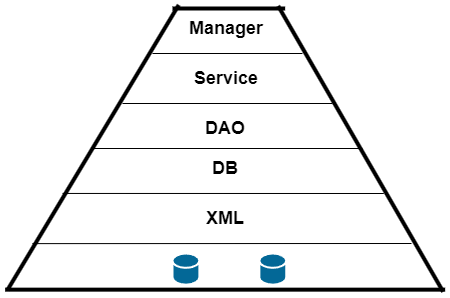
\includegraphics[width=0.6\columnwidth]{SchemaModel} 
    \bigskip
    \caption{Struttura Model CWBI}
\end{figure}

\noindent
Come detto in precedenza alcune delle classi già presenti sono state utilizzate per supportare le nuove entità introdotte con il progetto. Per la codifica del nostro nuovo Model ci siamo basati sulla figura \textit{5.4}, partendo dal basso e andando verso l'alto.  \\
\\
\noindent
Il primo passo per la creazione di una nuova classe è stato mappare i suoi attributi all'interno del file xml che conteneva la mappatura e specificava la struttura della tabella che sarebbe stata costruita poi sul database. \\
Prendiamo come esempio la classe Ticket. È stato creato il file \textit{\textbf{ticket.xml}} e all'interno è stata specificata la tabella \textit{ticket-a} con tutti gli attributi.\\
\\
\noindent
Dopo è avvenuta la codifica della classe \texttt{TicketDB.java} che rappresentava l'oggetto vero e proprio utilizzato nella  webapp. Importante specificare che gli attributi inseriti in questa classe erano uguali agli attributi specificati nella tabella   \textit{ticket-a} nel file di mappatura. La classe era composta quindi dagli attributi, i costruttori e le funzioni di \textit{get} degli attributi.\\
Le nomenclatura \textit{DB} dopo il nome della classe è uno standard dell'azienda inserito per ogni nuovo modello che si introduce.
\\
\noindent
Successivamente sono state create due classi: \texttt{\textbf{TicketDao}} e \texttt{\textbf{TicketDaoHibernate}}. \\
Partiamo con \textit{TicketDao} che rappresentava l'interfaccia in cui erano presenti le firme di tutte le funzioni per la manipolazione dei dati, secondo il pattern \textit{\textbf{Dao}}: le operazioni \textit{CRUD}. \\
La classe \texttt{TicketDaoHibernate} invece era l'implementazione dell'interfaccia \texttt{TicketDao}, che implementava quindi le funzioni presenti. \\
In realtà, l'esecuzione effettiva della funzione CRUD richiesta, non avveniva in \texttt{TicketDao-} \texttt{Hibernate} ma all'interno di ogni funzione implementata, veniva richiamata un'altra funzione con lo stesso scopo ma era implementata in un'altra classe \textit{Hibernate}, padre di \texttt{TicketDaoHibarnate} che 
effettuerà le operazioni classiche CRUD. \\
In generale, \texttt{TicketDaoHibarnate} implementava le funzioni dell'interfaccia a cui si riferiva, ma le operazioni CRUD erano sempre effettuate dall'\textit{Hibernate} padre.\\

\noindent
Il prossimo passo è stato creare le classi service: \texttt{\textbf{TicketService}} e \texttt{\textbf{TicketServiceImpl}}.\\
La classe \texttt{TicketService} era l'interfaccia al cui interno trovavamo le firme delle funzioni che la webapp consentiva di svolgere, come ad esempio la funzione di ricerca. \\
\texttt{TicketServiceImpl} invece era l'implementazione delle funzioni di \texttt{TicketService}. All'interno di ogni funzione, il dato veniva manipolato e alla fine, si richiamava la funzione della classe \texttt{TicketDao} specifica per il contesto. 
Si può dire che all'interno dell'implementazione di una funzione \textit{service} il dato era manipolato e personalizzato con l'obiettivo di fornire il risultato desiderato.\\

\noindent
Importante notare che la funzione di ricerca non era una funzione \textit{CRUD} e veniva implementata nel service. Infatti nella sua implementazione, questa funzione richiamava la funzione di \textit{TicketDaoHibernate} che avrebbe effettuato la \textbf{lettura} del dato corrispondete ai parametri di ricerca.\\

\noindent
Allora tutte le funzioni all'interno delle applicazioni si riducevano sempre a delle semplice funzioni \textit{\textbf{CRUD}}.\\

\noindent
L'ultima fase è stata creare le classi manager. Queste classi non sempre erano necessarie e fungevano da supporto per le classi service. \\
Nel progetto \textbf{non} sono state codificate classi manager.

\subsection*{Controller}
Lo scopo dei \textit{controller} all'interno dell'applicazione era quello di gestire le interazioni tra la parte di \textit{front-end} (View) e la parte di \textit{back-end} (Model), oltre a gestire anche gli input degli utenti.\\

\noindent
Il \textit{controller} aveva il compito di \textit{istanziare} le classi del Model, richiamarne le funzioni per avere un risultato e inviarlo poi al \textit{front-end} in modo da essere visualizzato.
All'interno dell'applicazione le classi che fungevano da \textit{controller} erano marcate dall'annotazione \textit{@Controller} di Spring.\\
Un'altra annotazione Spring presente era \textit{@Autowired} che serviva per indicare le dipendenze dei \textit{bean} (classi. Infatti all'interno dei controller si potevano trovare degli oggetti \textit{Service} utilizzati per le operazioni sul Model. Quindi, quando veniva istanziato il controller, si creavano anche gli oggetti all'interno di esso.\\

\noindent
\textit{CWBI} struttura i controller in due cartelle distinte. Prendiamo come esempio la classe Ticket del modello:\\

\textbf{Cartella Form}
\begin{itemize}
\item \texttt{TicketForm}: questa classe identificava i campi di input presenti alla creazione o alla modifica di un ticket, detti appunto \textit{Form}. Quindi quando l'utente compilava i campi, popolava gli attributi di questa classe. \\ Le caratteristiche di \texttt{TicketForm} dovevano essere adeguate alla controparte dell'oggetto Ticket nel modello. Infatti il \textit{controller} che si occupava della creazione e della modifica, aveva il compito di costruire l'oggetto Ticket partendo dall'oggetto TicketForm appena popolato. 

\item \texttt{TicketSearchForm}: questa classe identificava i campi di input presenti alla ricerca di un ticket. L'utente per effettuare la ricerca di un ticket poteva scegliere o compilare dei filtri , rappresentati da \texttt{TicketSearchForm}. \\
Le caratteristiche di tale classe erano redatte in base ai tipi di filtri che si volevano fornire all'utente e dovevano essere adeguati per le proprietà dell'oggetto su cui si stava effettuando la ricerca.

\end{itemize}
\medskip

\textbf{Cartella Action} 
\begin{itemize}
\item[] Le classi presenti in questa cartella, sono dette \textit{Action} ed erano i veri e propri \textit{controller} che svolgevano le varie funzioni.

\item \textttTicketAction}: come si può leggere, la classe non presenta la nomenclatura \textit{Form}. Infatti questa \textit{Action} si occupava di gestire le pagine della webapp che non possedevano form al loro interno. Il dettaglio del Ticket era gestito da \texttt{TicketAction} in quanto non possedeva nessun tipo di campo da compilare.\\
Erano presenti diverse funzioni, come ad esempio la funzione di caricamento della pagina di dettaglio di un Ticket. In questa funzione veniva utilizzato l'oggetto \texttt{TicketService} per richiamare la funzione di ricerca per id e trovare l'oggetto \textit{Ticket} corrispondente e stampare i dati a schermo.

\item \texttt{TicketFormAction}: questo \textit{controller} si occupava di gestire le \textit{Action} che riguardano la pagina di creazione e modifica di un \textit{Ticket} attraverso la manipolazione dell'oggetto \texttt{TicketForm}. Prendiamo come esempio la creazione di un nuovo Ticket.\\
Quando si entrava nella pagina di creazione di un ticket, i campi dell'oggetto \texttt{TicketForm} erano inizializzati vuoti dall'Action \textit{input} e dovevano essere compilati dall'utente. Al salvataggio, veniva richiamata un'altra \textit{Action} che si occupava di prendere i valori presenti nell'oggetto\texttt{TicketForm} e creare un nuovo oggetto \textit{Ticket} con i dati prelevati.\\ Alla fine, si utilizzava l'oggetto\texttt{TicketService} per salvere il nuovo oggetto \textit{Ticket}.

\item \texttt{TicketSearchFormAction}: l'ultimo \textit{controller} era utilizzato per le pagine di ricerca di un ticket e utilizzava l'oggetto \texttt{TicketSearchForm} per le proprie funzionalità. Quando si entrava nella pagina di ricerca, i campi dell'oggetto\texttt{TicketSearchForm} che rappresentavano i filtri di ricerca, erano inizializzati vuoti ed era l'utente poi a riempirli. Quando si effettuava la ricerca, veniva richiamata la \textit{Action} di \textit{search}, dove si costruiva un nuovo oggetto \textit{Ticket} a seconda delle caratteristiche (filtri) dell'oggetto \texttt{TicketSearchForm}. \\
Veniva quindi utilizzato l'oggetto \texttt{TicketService} per richiamare la funzione di ricerca che prendeva in input un oggetto \textit{Ticket} e confrontava quale dei ticket presenti nel database aveva i valori uguali a quelli del ticket passato. Venivano così trovati tutti i ticket corrispondenti ai filtri inseriti.
\end{itemize}

\subsection*{View}
L'ultimo componente dell'architettura era la \textit{\textbf{View}} che aveva il compito di visualizzare i dati secondo una logica e fornire la possibilità all'utente di interagire con il modello.
\\
\noindent
Le pagine che componevano la webapp erano file \textit{jsp} che permettevano di scrivere codice con standard HTML o XML, ma anche di integrare le funzionalità di Java rendendo i contenuti dinamici. \\
\newpage
\noindent
La \textbf{\textit{View}} era supportata anche da diversi \textit{framework} come \textit{Bootstrap} che forniva delle classi per personalizzare il contenuto della pagina andando a codificare tali classi direttamente nel attributo "class" dei tag di HTML. \\
Alle pagine jsp era affiancata un'estensione detta \textit{JSTL} che mette a disposizione dei tag per la visualizzazione dei dati in modo dinamico.
\\
\noindent
Per l'interazione tra modello, controller e view entrava in gioco un'ulteriore \textit{framework}, senza il quale, non era possibile il funzionamento della webapp cos' com'è stata pensata e codificata da CWBI: \textit{\textbf{Struts}}.\\

\noindent
L'utente, nell'utilizzo della webapp, interagiva con gli elementi messi a disposizione dalla \textit{View} e richiamava delle specifiche \textit{Action} di controller specifici. Questa interazione era possibile grazie a \textit{Struts} che permetteva di associare un file jsp ad una Action di un controller, andando a configurare il file \textit{struts.xml}.

\section{Design Pattern}
I \textbf{\textit{Design Pattern}} sono soluzioni generali utilizzate per risolvere problemi ricorrenti durante lo sviluppo di un'applicazione. Esistono diversi \textit{design pattern} ed ognuno di loro ha uno scopo preciso durante la codifica del prodotto. \\
Possiamo riconoscere tre famiglie per i \textit{design pattern}:\\
\begin{itemize}
\item \textbf{Comportamentali}: definiscono le interazioni tra gli oggetti e distribuiscono le responsabilità.
\item \textbf{Creazionali}: si occupano di come creare gli oggetti
\item \textbf{Strutturali}: provvedono a definire la struttura delle classi, degli oggetti e come essi sono composti.
\end{itemize} 
\\
\noindent
L'azienda \textit{CWBI} ha applicato i seguenti \textit{design pattern} per la codifica delle loro applicazioni. Tali pattern sono anche presenti nel progetto in quanto basato su una struttura ben definita e solida.

\subsection*{Dependency Injection}
La \textit{Dependency injection} è una tecnica che si occupa di separare la creazione di un oggetto dal suo effettivo utilizzo. Quindi quando un oggetto vuole utilizzare un servizio/oggetto, non deve preoccuparsi di come questo servizio/oggetto è composto o creato in quanto li verrà \textit{iniettato} dall'esterno. Quindi le dipendenze di un oggetto con i componenti o i servizi che lo compongono sono risolte e iniettate da una classe chiamata \textbf{\textit{Injectors}}.\\
Questo \textit{pattern} porta ad avere vantaggi come il riutilizzo, la testabilità e la manutenzione del codice. 
\newpage
\subsection*{Inversion of Control}  
L' \textbf{\textit{Inversion of Control}}, detto anche \textbf{\textit{IoC}} è un design pattern molto importante ed è uno dei modi per applicare la \textit{dependency injection}.\\
Normalmente il flusso di un'applicazione è determinato dagli oggetti e quindi dal codice che la compongono. Con \textit{IoC} il controllo del flusso è affidato ad un \textit{framework} che si occuperà degli oggetti e delle loro dipendenze.\\
Un esempio di framework che applica \textit{IoC} è \textit{Spring} che introduce delle annotazioni come: \textit{@Component}, \textit{@Service}, \textit{@Repository} o \textit{@Controller}.

\subsection*{Decorator}
 \begin{figure}[H]
    \centering 
    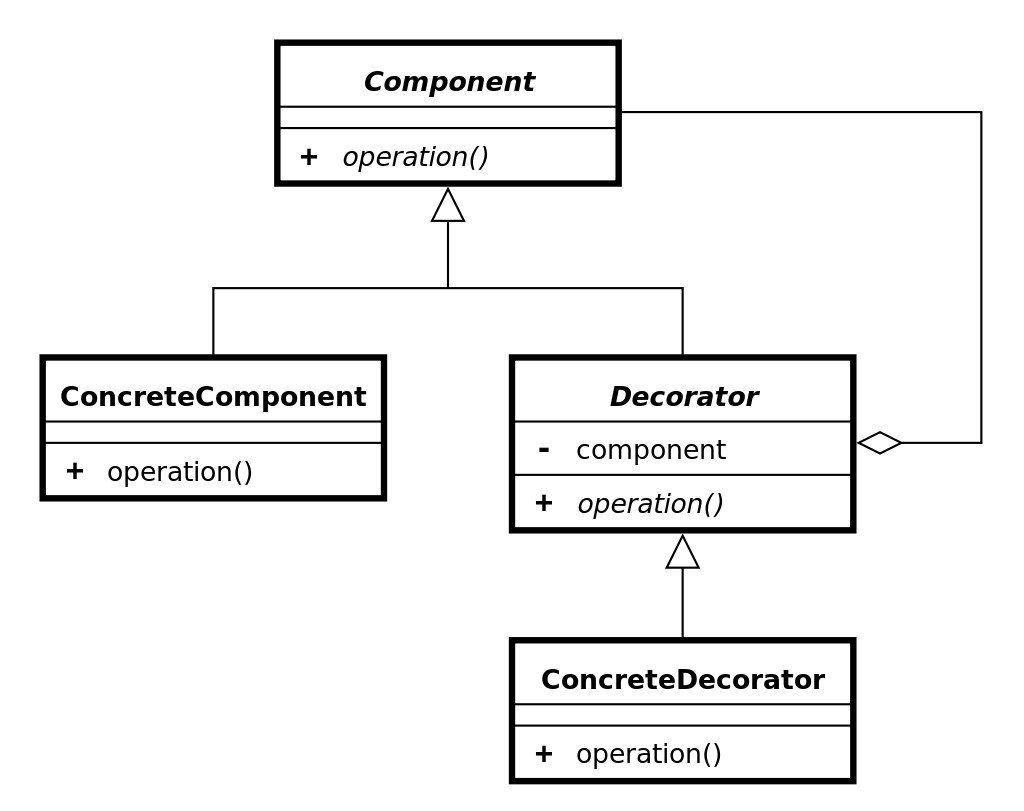
\includegraphics[width=0.6\columnwidth]{decorator} 
    \bigskip
    \caption{Pattern decorator}
\end{figure}

Il pattern \textit{\textbf{Decorator}} è un pattern strutturale che permette di introdurre nuove funzionalità e comportamenti ad un oggetto senza cambiarne la struttura. L'introduzione di questi nuovi elementi viene effettuata a \textit{run-time}.
Come si vede dalla \textit{figura 5.5} gli elementi che compongono il \textit{decorator} sono:
\begin{itemize}
\item \textbf{Component}: rappresenta l'interfaccia dell'oggetto da creare;
\item \textbf{ConcreteComponent}: è l'oggetto a cui verranno aggiunte le nuove caratteristiche;
\item \textbf{Decorator}: è l'interfaccia dei Decorator che aggiungeranno le nuove funzioni;			 
\item \textbf{ConcreteDecorator}: rappresenta gli oggetti Decorator che hanno il compito di aggiungere le nuove funzionalità al \textit{ConcreteComponent}. 
\end{itemize}
\subsection*{Data Access Object}
 \begin{figure}[H]
    \centering 
    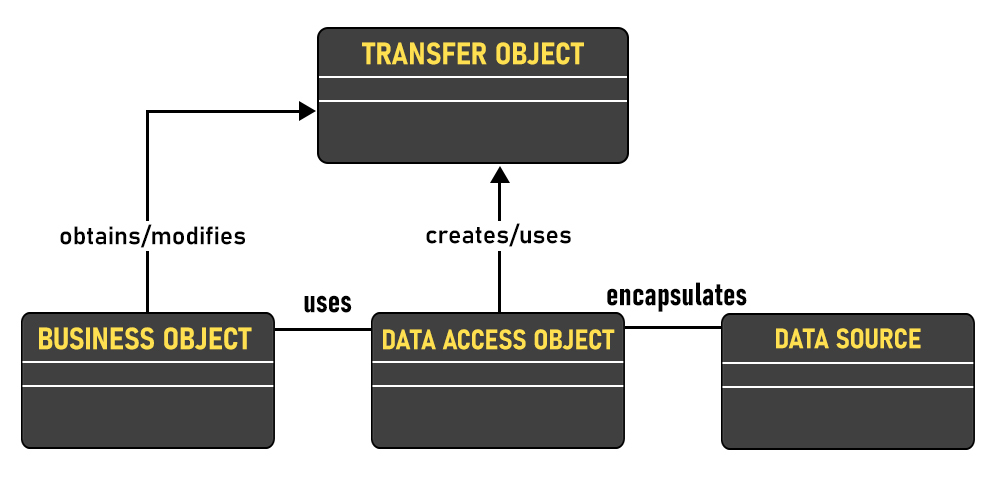
\includegraphics[width=0.7\columnwidth]{DAO} 
    \bigskip
    \caption{Pattern DAO}
\end{figure}
Il pattern \textit{\textbf{Data Access Object}}, detto anche \textit{\textbf{Dao}}, è un pattern architetturale che permette di dividere il livello di business dell'applicazione dalla fonte da cui arrivano i dati, per esempio un database. \\
Mette a disposizione un'interfaccia che mappa le operazione sui dati alle chiamate per il database. In generale, facilita l'utilizzo delle funzioni \textit{CRUD} separando i bisogni dell'applicazione dal come questi bisogni dovranno essere soddisfatti. In questo modo il livello business e il database evolveranno separatamente senza conoscere i dettagli l'uno dell'altro.
